
\documentclass[crop,tikz]{standalone}
\usepackage[utf8]{inputenc}
\usepackage{tikz}
\usepackage{pgfplots}
\pgfplotsset{compat=newest}
\usepgfplotslibrary{groupplots}
\begin{document}
% This file was created by matplotlib2tikz v0.6.15.
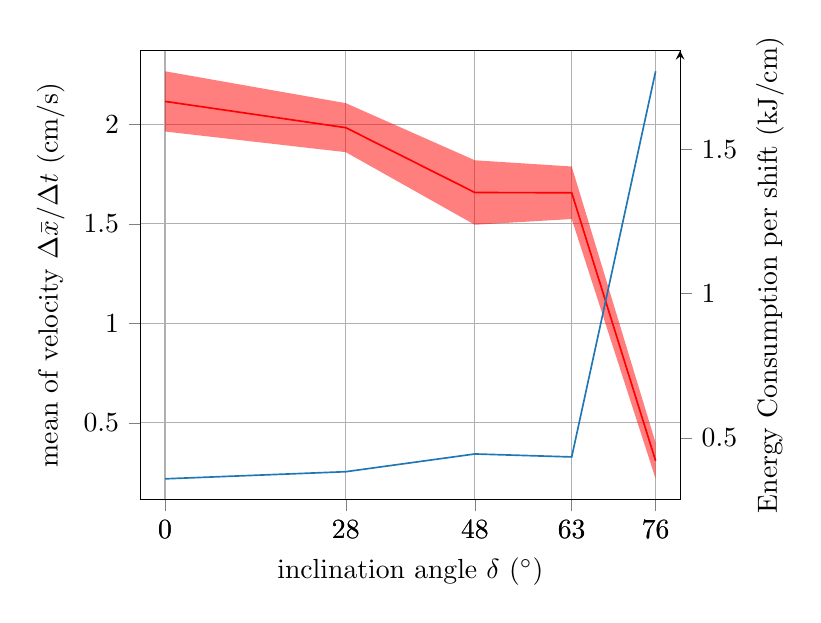
\begin{tikzpicture}

\definecolor{color0}{rgb}{0.12156862745098,0.466666666666667,0.705882352941177}

\begin{axis}[
xlabel={inclination angle $\delta$ ($^\circ$)},
ylabel={mean of velocity $\Delta \bar{x} / \Delta t$ (cm/s)},
xmin=-3.8, xmax=79.8,
ymin=0.116151651087804, ymax=2.3692414509782,
tick align=outside,
tick pos=left,
xmajorgrids,
x grid style={lightgray!92.026143790849673!black},
ymajorgrids,
y grid style={lightgray!92.026143790849673!black},
xtick={0, 28, 48, 63, 76}
]
\path [fill=red, fill opacity=0.5] (axis cs:0,1.96397628120578)
--(axis cs:0,2.26682827825591)
--(axis cs:28,2.10657374096983)
--(axis cs:48,1.81945582918713)
--(axis cs:63,1.78819413913446)
--(axis cs:76,0.399527687236154)
--(axis cs:76,0.218564823810095)
--(axis cs:76,0.218564823810095)
--(axis cs:63,1.524299015765)
--(axis cs:48,1.49540749485268)
--(axis cs:28,1.86018787290638)
--(axis cs:0,1.96397628120578)
--cycle;

\addplot [semithick, red, forget plot]
table {%
0 2.11540227973084
28 1.9833808069381
48 1.6574316620199
63 1.65624657744973
76 0.309046255523125
};
\end{axis}

\begin{axis}[
ylabel={Energy Consumption per shift (kJ/cm)},
xmin=-3.8, xmax=79.8,
ymin=0.287415789177992, ymax=1.84151804675822,
axis y line=right,
tick align=outside,
xtick pos=left,
ytick pos=right,
x grid style={lightgray!92.026143790849673!black},
y grid style={lightgray!92.026143790849673!black},
xtick={0, 28, 48, 63, 76}
]
\addplot [semithick, color0, forget plot]
table {%
0 0.358056800886184
28 0.382742479374471
48 0.444272094725907
63 0.433909221622489
76 1.77087703505003
};
\end{axis}

\end{tikzpicture}
%% End matplotlib2tikz content %% 
\end{document}